\documentclass{beamer}

\usepackage[super]{nth}		% Per rappresentare numericamente first, second, ecc.


\title{HVAC Waste Detection - Project Presentation}
\author{Daniele Polidori}
\institute{\textit{Course of Internet of things}\\
\textit{University of Bologna}}
\date{Academic year 2023-24}

\setbeamertemplate{navigation symbols}{\tiny\insertframenumber}     % Inserisce il numero di pagina al posto dei simboli di navigazione
\setbeamercolor{navigation symbols}{fg=black}   % Colora di nero i simboli di navigazione


\begin{document}


{
\setbeamertemplate{footline}{}      % Elimina il footline in questa slide
\setbeamertemplate{navigation symbols}{}    % Lascia uno spazio vuoto al posto dei simboli di navigazione
\begin{frame}
 \titlepage     % Beamer's \maketitle
\end{frame}
}
%\addtocounter{framenumber}{-1}     % Non considera questa slide nel conteggio delle pagine


\begin{frame}{IoT system}

	It \textbf{monitors} the temperature of an house, to prevent useless HVAC consumption, detecting it by rapid \textbf{temperature changes}.
	
	\vfill

	\begin{block}

		\begin{columns}[onlytextwidth,T]
		
			\column{\dimexpr\linewidth-60mm-5mm}

			Composed by an \textbf{ESP-WROOM-32} board linked to:
			\begin{itemize}
				\item 1 \textbf{indoor DHT22},
				\item 1 \textbf{outdoor DHT22},
				\item 1 \textbf{LED}.
			\end{itemize}

			\column{60mm}
			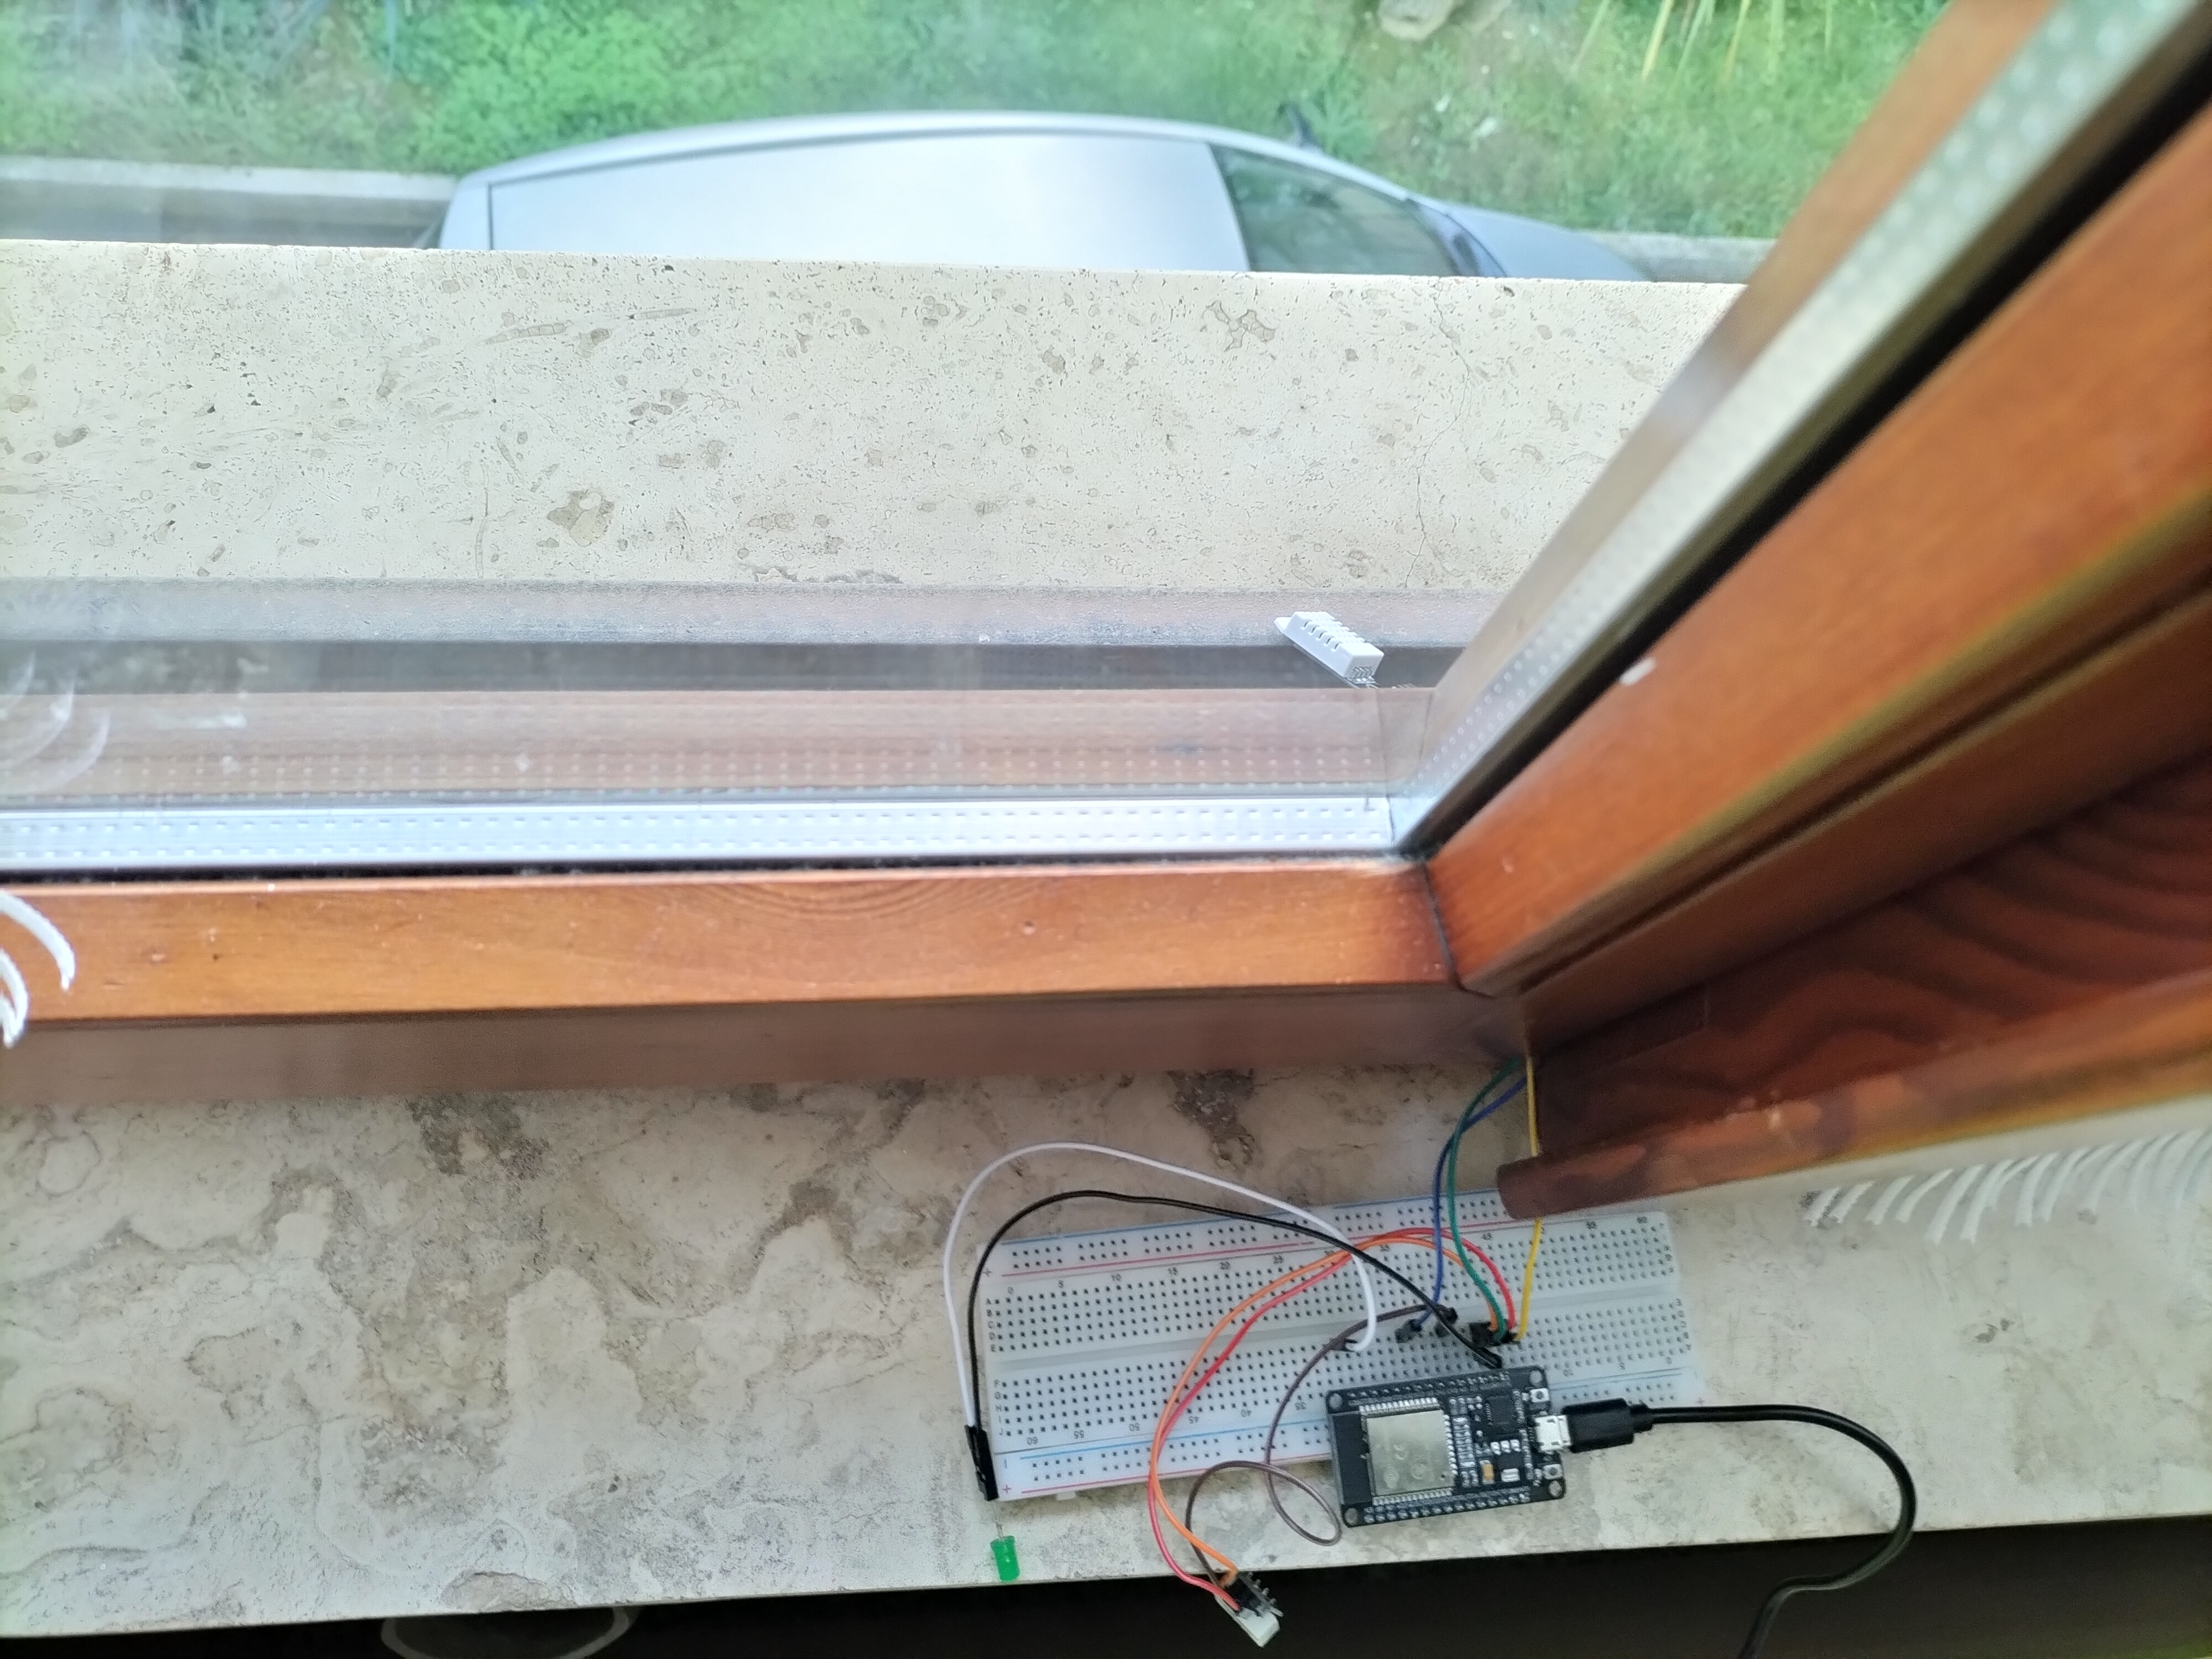
\includegraphics[scale=0.04]{figures/figure_esp.jpg}

		\end{columns}
	\end{block}
\end{frame}


\begin{frame}{Data acquisition - ESP32}

	\begin{description}[\texttt{PubSubClient}]		% Indico la lunghezza della label piu' lunga, cosi' che siano tutte allineate a dx
		\item[\texttt{Thing.CoAP}]: to act as a \textbf{CoAP server}.
		\item[\texttt{PubSubClient}]: to act as a \textbf{MQTT subscriber}.
	\end{description}

	\vfill

	Through \textbf{CoAP}, the ESP32 is able to \textbf{send} the latest collected indoor and outdoor temperature value, \textbf{when asked}.

	\vfill

	Through \textbf{MQTT}, the board \textbf{can receive} some \textbf{commands}:
	\begin{itemize}
		\item to start or stop the \textbf{sensors reading},
		\item to change their \textbf{sampling rate},
		\item to turn on or off the \textbf{LED}.
	\end{itemize}
	My laptop acts as a MQTT broker, through Mosquitto.

\end{frame}


\begin{frame}{Data proxy - \nth{1} Python script}

	\begin{description}[\texttt{influxdb-client}]		% Indico la lunghezza della label piu' lunga, cosi' che siano tutte allineate a dx
		\item[\texttt{paho-mqtt}]: to act as a \textbf{MQTT publisher}.
		\item[\texttt{aiocoap}]: to act as a \textbf{CoAP client}.
		\item[\texttt{influxdb-client}]: to \textbf{store} data.
	\end{description}

	\vfill

	\textbf{Initially}, through \textbf{MQTT}, the application gives commands, to the ESP32, to \textbf{start} the sensors reading and to set their \textbf{sampling rate}.
	
	\vfill
	
	\textbf{Periodically}, through \textbf{CoAP}, the script \textbf{requests}, to the board, the latest collected indoor and outdoor temperature value.\\
	It \textbf{continuously stores} these values on a local InfluxDB instance.
	
	\vfill
	
	The network \textbf{latency}, between the temperature value request and its reception, is continuously monitored and, after a while from the beginning, the mean value is calculated.

\end{frame}


\begin{frame}{Data analytics - \nth{2} Python script (1/2)}

	\begin{description}[\texttt{influxdb-client}]		% Indico la lunghezza della label piu' lunga, cosi' che siano tutte allineate a dx
		\item[\texttt{influxdb-client}]: to \textbf{get} and \textbf{store} data.
		\item[\texttt{prophet}]: to \textbf{forecast} future temperature values.
		\item[\texttt{paho-mqtt}]: to act as a \textbf{MQTT publisher}.
	\end{description}

	\vfill

	At the \textbf{beginning}, the script gets all past temperature values to \textbf{forecast} some indoor and outdoor values.\\As the times are reached, the application \textbf{stores} the predicted values on the database.
	
	\vfill
	
	\textbf{Ciclically}, the application retrieves some of the latest temperature values and \textbf{analyses} them to check a possible HVAC waste.\\
	When the alarm \textbf{goes off}, the script \textbf{stores} the event on the database and, through \textbf{MQTT}, gives the command, to the ESP32, to turn on the \textbf{LED}; when the risk has passed, the script gives the command to turn it off.

\end{frame}


\begin{frame}{Data analytics - \nth{2} Python script (2/2)}

	The alarm \textbf{goes off} if:
	\begin{itemize}
		\item the indoor temperature is \textbf{changing} rapidly \eqref{eq_varianza} and
		\item the indoor temperature is \textbf{approaching} the outdoor one \eqref{eq_media}.
	\end{itemize}
	
	\vfill
	
	Mathematically speaking:
	\begin{equation}
	var(i_1, i_2, \dots, i_n) > threshold \label{eq_varianza}
	\end{equation}
	\begin{equation}
	min(i_n, o_n) < mean(i_1, i_2, \dots, i_n) < max(i_n, o_n) \label{eq_media}
	\end{equation}
	where $i$ is the indoor temperature, $o$ is the outdoor temperature and $t_1, t_2, \dots, t_n$ are the $n$ latest temperature values retreived: $t_1$ is the newest and $t_n$ is the farthest.

\end{frame}


\begin{frame}{Data visualization}

 	Local \textbf{Grafana} instance that shows:
	\begin{block}

		\begin{columns}[onlytextwidth,T]
		
			\column{\dimexpr\linewidth-65mm-5mm}

			\begin{itemize}
				\item the \textbf{collected} temperature values,
				\item the \textbf{forecasted} ones,
				\item the counting of the \textbf{alarm} events.
			\end{itemize}

			\column{70mm}
			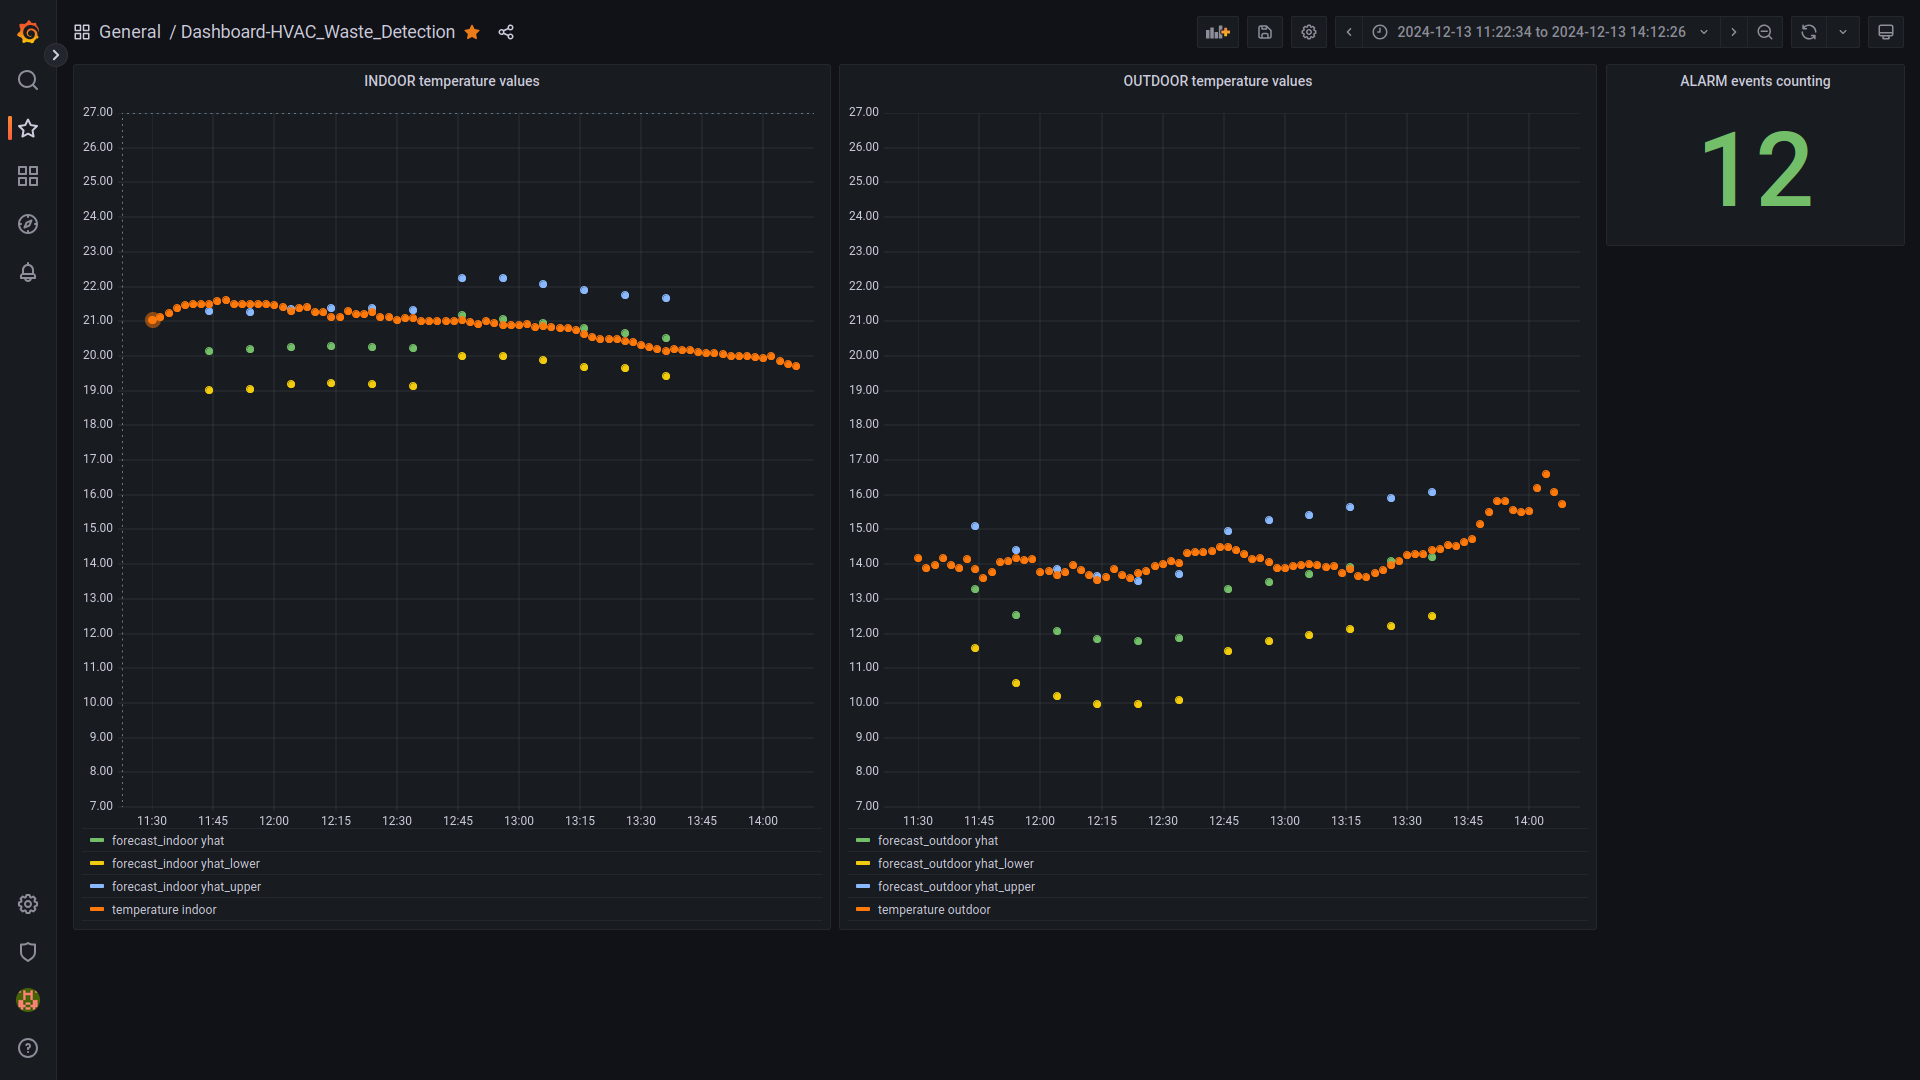
\includegraphics[scale=0.10]{figures/figure_grafana.png}

		\end{columns}
	\end{block}
\end{frame}


\begin{frame}{Setup - Data proxy}

	ESP32)
	\begin{description}[Mean network latency evaluation]
		\item[\textbf{Indoor} DHT sampling rate]: 3 sec.
		\item[\textbf{Outdoor} DHT sampling rate]: 20 sec.
	\end{description}
	
	\vfill
	
	Data acquisition process)
	\begin{description}[Mean network latency evaluation]
		\item[Latest \textbf{temperatures} request]: every 5 sec.
		\item[Mean network \textbf{latency} evaluation]: after 1 hour.
	\end{description}

\end{frame}


\begin{frame}{Setup - Data analytics}

	Forecast)
	\begin{description}[Num. of values retreived]
		\item[Data \textbf{obtained}]: on start.
		\item[Temperatures \textbf{collection}]: past month (unevenly).
		\item[\textbf{aggregate}Window]: every 20 sec (mean function).
		\item[Num. of values \textbf{retreived}]: 6500 indoor, 6500 outdoor.
		\item[Values \textbf{forecasted}]: every 10 min, for 6 times.
	\end{description}
	
	\vfill
	
	Alarm)
	\begin{description}[Num. of values retreived]
		\item[Data \textbf{obtained}]: every 30 sec.
		\item[Temperatures \textbf{collection}]: latest 2 min.
		\item[Alarm \textbf{threshold} \eqref{eq_varianza}]: $0.03$ $^\circ \text{C}^2$.
	\end{description}

\end{frame}


\begin{frame}{Evaluation}

	\begin{description}[Mean network latency]
		\item[Day]: on December 13th.
		\item[Data \textbf{proxy} started]: at 11:30.
		\item[Data \textbf{analytics} started]: at 12:36.
	\end{description}
	
	\vfill
	
	\begin{description}[Mean network latency]
		\item[Mean network \textbf{latency}]: $150$ millis (ranging from $5$ to $421$).
	\end{description}
	
	\vfill
	
	\begin{description}[Max difference outdoor forecasted-observed]
		\item[Max difference \textbf{indoor} forecasted-observed]: $0.39$ °C.
		\item[Max difference \textbf{outdoor} forecasted-observed]: $1.23$ °C.
	\end{description}
	(Always within the forecasted range.)

\end{frame}


\begin{frame}{Results - Indoor forecast}

	\begin{table}[htbp]\small
		\begin{center}
			\begin{tabular}{|r||c||c|c|c|}
				\hline
				\textbf{Current} & \textbf{Observed}$^{\mathrm{a}}$ & \multicolumn{3}{|c|}{\textbf{Forecasted Temperature (°C)}} \\
				\cline{3-5}
				\textbf{Time} & \textbf{Temperature (°C)} & \textbf{yhat} & \textbf{yhat lower} & \textbf{yhat upper} \\
				\hline
				\hline
				12:46 & $21.04$ & \textbf{21.17} & $19.99$ & $22.25$ \\
				\hline
				12:56 & $20.88$ & \textbf{21.07} & $19.98$ & $22.24$ \\
				\hline
				13:06 & $20.85$ & \textbf{20.95} & $19.88$ & $22.06$ \\
				\hline
				13:16 & $20.63$ & \textbf{20.81} & $19.69$ & $21.90$ \\
				\hline
				13:26 & $20.42$ & \textbf{20.66} & $19.66$ & $21.77$ \\
				\hline
				13:36 & $20.13$ & \textbf{20.52} & $19.43$ & $21.67$ \\
				\hline
				\multicolumn{4}{l}{$^{\mathrm{a}}$Mean temperature value (of the 2 minutes around).}
			\end{tabular}
			\label{tab_forecast_indoor}
		\end{center}
	\end{table}
\end{frame}


\begin{frame}{Results - Outdoor forecast}

	\begin{table}[htbp]\small
		\begin{center}
			\begin{tabular}{|r||c||c|c|c|}
				\hline
				\textbf{Current} & \textbf{Observed}$^{\mathrm{a}}$ & \multicolumn{3}{|c|}{\textbf{Forecasted Temperature (°C)}} \\
				\cline{3-5}
				\textbf{Time} & \textbf{Temperature (°C)} & \textbf{yhat} & \textbf{yhat lower} & \textbf{yhat upper} \\
				\hline
				\hline
				12:46 & $14.50$ & $13.27$ & $11.49$ & \textbf{14.97} \\
				\hline
				12:56 & $14.07$ & \textbf{13.49} & $11.78$ & $15.26$ \\
				\hline
				13:06 & $14.01$ & \textbf{13.71} & $11.95$ & $15.42$ \\
				\hline
				13:16 & $13.86$ & \textbf{13.92} & $12.13$ & $15.65$ \\
				\hline
				13:26 & $13.98$ & \textbf{14.09} & $12.21$ & $15.91$ \\
				\hline
				13:36 & $14.40$ & \textbf{14.21} & $12.49$ & $16.09$ \\
				\hline
				\multicolumn{4}{l}{$^{\mathrm{a}}$Mean temperature value (of the 2 minutes around).}
			\end{tabular}
			\label{tab_forecast_outdoor}
		\end{center}
	\end{table}
\end{frame}


\begin{frame}{Considerations}

	Little \textbf{more reliable} in forecasting the \textbf{indoor} temperature.\\
	It can be due to the \textbf{higher sampling rate} of the indoor sensor (useful to rapidly detect an eventual HVAC waste, unnecessary outdoor).
	
	\vfill
	
	The experiment done has \textbf{limitations}:
	\begin{itemize}
		\item \textbf{not many} past temperature \textbf{values} available,
		\item temperature data \textbf{collected unevenly};
		\item \textbf{ESP32} was \textbf{positioned} in a naive way (e.g. it should be arranged in such a way as to avoid direct sunlight).
	\end{itemize}

\end{frame}


\end{document}
